\centering
\underline{\textsc{The Pocket Rules}}

\vspace*{1em}
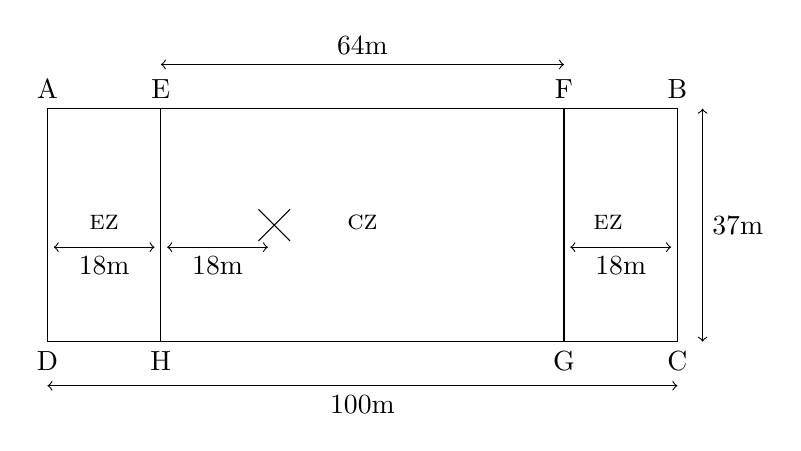
\begin{tikzpicture}[scale=0.08]
  % Draw field outline
  \draw (0,0) rectangle (100,37);

  % Draw goal areas
  \draw (0,0) rectangle (18,37);
  \draw (82,0) rectangle (100,37);

    % brick mark
  \draw (33.5,16) -- (38.5,21);
  \draw (38.5,16) -- (33.5,21);


  % length arrows
  \draw[<->] (0,-7) -- (100,-7) node[midway, below] {100m};
  \draw[<->] (19,15) -- (35,15) node[midway, below] {18m};
  \draw[<->] (1,15) -- (17,15) node[midway, below] {18m};
  \draw[<->] (83,15) -- (99,15) node[midway, below] {18m};
  \draw[<->] (18,44) -- (82,44) node[midway, above] {64m};
  \draw[<->] (104, 0) -- (104, 37) node[midway, right] {37m};


  % labels
  \node at (0,37) [above] {A};
  \node at (18,37) [above] {E};
  \node at (82,37) [above] {F};
  \node at (100,37) [above] {B};
  \node at (0,0) [below] {D};
  \node at (18,0) [below] {H};
  \node at (82,0) [below] {G};
  \node at (100,0) [below] {C};

    \node at (50,19) {\sc cz};
    \node at (9,19) {\sc ez};
    \node at (89,19) {\sc ez};
\end{tikzpicture}
\vspace*{-1.5cm}
\begin{multicols}{2}
    \[\{AB, BC, CD, DA\} \not \subset \text{field}\]\tab{}\[\{EH, FG\} \not \subset \text{EZ}\]
\end{multicols}


{\small{\textgreek{ἀγεωμέτρητοσ μηδεὶσ εἰσίτω}}}

\begin{center}[0]\end{center}
